\title{A pilot study examining the diet of introduced Alaska blackfish (\textit{Dallia pectoralis} T.\ H.\ Bean, 1880) in Kenai, Alaska, by metabarcoding}

\subtitle{\doi{10.----------}}

\author{by Matt Bowser\footnote{US Fish \& Wildlife Service, Kenai National Wildlife Refuge, Soldotna, Alaska, \email{Matt\_Bowser@fws.gov}}and Apphia Bowser}

\maketitle

\end{multicols}
\begin{figure}[H]
\begin{center}
%\vspace{2mm}
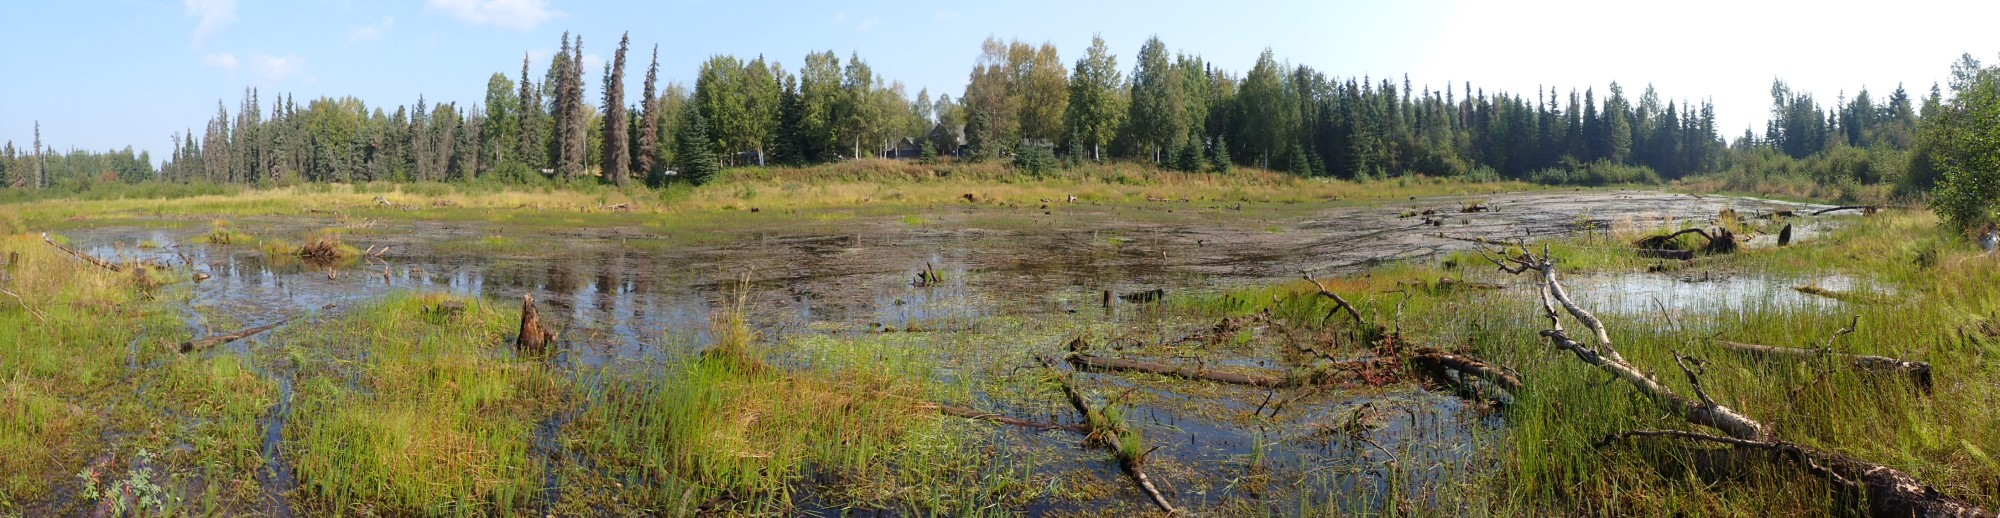
\includegraphics[width=\textwidth]{img/blackfish_pond.jpg}
\caption{Panoramic montage of a pond off of the Kenai Spur Highway and Candlelight Drive, the locality from which blackfish specimens were collected. A full resolution image is available on Arctos (\doi{10.7299/X7ZP46FP}).}
\label{blackfish_pond}
\end{center}
\end{figure} 
\begin{multicols}{2}   

\section{Introduction}

Last year we  wrote about some food items of the Alaska blackfish, \textit{Dallia pectoralis} T.\ H.\ Bean, 1880 \citep{Bowseretal2019},  a fish species that is native to part of Alaska, but not the Kenai Peninsula. We wanted to learn more about how these introduced fish may alter the ecology of Kenai Peninsula waters, especially how blackfish may affect native fish species through competition for invertebrate prey.

\section{Methods}

On August 23, 2019, we author collected blackfish from a small, shallow pond in Kenai, Alaska (60.5681~\textdegree{}N, -151.1901~\textdegree{}W $\pm$ 40~m) \citep{bowser2019}, the same pond from which we had obtained blackfish the previous year. This pond (Figure \ref{blackfish_pond}) is fed by a small inlet stream and its level is maintained by a dam at the outlet. There is little open water; most of the pond is thickly filled with \textit{Potamogeton} and flocculent iron bacterial scum. Only one other fish species, a single specimen of a nine-spined stickleback (\textit{Pungitius pungitius} (Linnaeus, 1758),  
\url{https://www.inaturalist.org/observations/31561030}), was observed in this pond.

We attempted to collect blackfish from other reaches of the stream, but found only small juveniles. 

The collected blackfish were placed on ice in a cooler, transported to the lab, and frozen. Later we thawed five adult blackfish, measured their lengths, dissected out their entire guts, and squeezed gut contents into vials of UniGard -100 propylene glycol antifreeze.

Vials of gut contents were shipped to \acr{RTL} Genomics in Lubbock, Texas (\url{https://rtlgenomics.com/}) for RTL Genomics' standard microbial diversity assay using the \textit{mlCOIint}/\textit{jgHCO2198} (GGWACWGGWTGAACWGTWTAYCCYCC/TAIACYTCIGGRTGICCRAARAAYCA) primer set.

Extraction methods, sequencing methods, and resulting raw sequence data are provided in \citet{BowserBowser2020}.

Raw reads were processed using the \acr{SCVUC} \acr{COI} metabarcode pipeline version 4.3.0 (\url{https://github.com/Hajibabaei-Lab/SCVUC_COI_metabarcode_pipeline}). This pipline runs SeqPrep \citep{StJohn2016}, \acr{CUTADAPT} \citep{Martin2011}, \acr{VSEARCH} \citep{Rognes2016}, \acr{UNOISE} \citep{Edgar2016}, and the RDP classifier \citep{Wang2007} using the \acr{COI} Classifier v4 reference dataset \citep{PorterHajibabaei2018}. All processing steps are run via Snakemake \citep{KosterRahmann2012}. Our \acr{SCVUC} configuration file \citep{Bowser2020config} and snakefile \citep{Bowser2020snakefile} are available on Arctos.

The resulting exact sequence variants (\acr{ESV}s) were also compared to \acr{ESV}s obtained by \citet{Bowseretal2020} \citep[dataset: ][]{, Bowseretal2020sup5}, sequences from the Alaska terrestrial arthropod \acr{DNA} barcode \acr{COI} reference library (\url{https://github.com/mlbowser/AKTerrInvCOILib}), and a \acr{FASTA} file of sequences from the authors' LifeScanner (\url{http://lifescanner.net/}) records (\url{http://www.boldsystems.org/index.php/Public_SearchTerms?query=DS-BOWSER}) using \verb|vsearch --usearch_global|. We also submitted our \acr{ESV}s to \acr{BLAST} and \acr{BOLD} \acr{ID} Engine searches and scrutinized the results. We followed the guidlines of \citet{Sigovinietal2016} when assigning provisional names.

We removed all reads identified as \textit{Dallia pectoralis}; \textit{Bos taurus} Linnaeus, 1758; and all non-animals. The small numbers of \textit{Bos taurus} reads likely came from bovine serum albumin added during \acr{DNA} amplification. As a final check of identifications, we generated a phylogeny of the filtered \acr{ESV}s using NGPhylogeny.fr, ``NGPhylogeny Analyse - FastME/OneClick'' option \citep{DesperGascuel2002, CriscuoloGribaldo2010, JunierZdobnov2010, KatohStandley2013, Lefortetal2015, Lemoineetal2019} and examined the tree using i\acr{TOL} \citep{LetunicBork2019}. The \acr{FASTA} file of retained \acr{ESV} sequences is available from Arctos \citep{Bowser2020bfdfas} and the phylogentic tree is available at \url{https://itol.embl.de/tree/16415961276811585237767}. 

To prevent reporting false postive occurrences, we removed occurrences represented by $\leq 0.05\%$ of the total number of reads of an \acr{ESV}. Complete analysis details are provided in \citet{bowser2020}.

We tried to follow the guidelines of \citet{Penevetal2017} by publishing occurrence data on Arctos, which supplies occurrence data to \acr{GBIF}. Specimen records, images, and other related files have been made available via an Arctos project at \url{http://arctos.database.museum/project/10003367}.

\section{Results}

\section{Discussion}

It was surprising that we detected none of the food items documented by \citet{Bowseretal2019}.

\section{Acknowledgments}

We thank Mike Baldwin for reviewing our list of potential new distribution records and pointing out that \textit{Angarotipula illustris} (Doane, 1901) was already known to occur in Alaska \citep{Brodo2018}.

\bibliography{blackfish_diet}


